\section{Cell assembly detection method}
\label{chap:AssemblyMethod}
%\subsection{Introduction}
On the described data-set we applied a cell assembly detection method developed in our lab (\cite{RussoDurstewitz}), that we present in this section to facilitate reading and interpretation of analysis results.\\
The first cell assembly definition was given by \cite{Hebb} a cell assembly is described as a group of neurons which, by functionally organizing into a temporally coherent set, come to represent mental or perceptual entities, thereby forming the basis of neural coding and computation. Such not stringent definition has resulted in a broad use of the term cell-assembly, that denotes in fact anything from the precise zero-phase-lag spike synchronization in a defined subset of neurons (\cite{Abeles}; \cite{Singer}; \cite{Roelfsema}; \cite{Diesmann}; \cite{Harris2003}) to temporally coherent changes in average firing rates on larger time scales (\cite{Goldman}; \cite{Durstewitz}).\\Which implies that the type of the detected assembly depends on the definition of the degree of temporal precision and coordination, in fact varying those definition is possible to detect a plethora of spike patterns, as is shown in fig.\ref{fig:CellAsseDet} \\
\begin{figure}
    \centering
    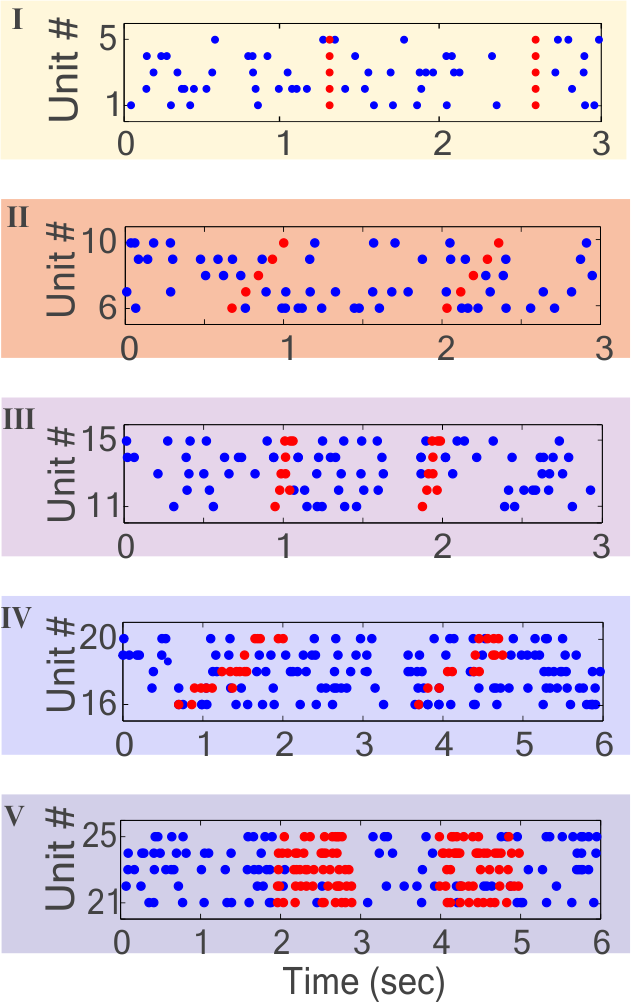
\includegraphics[scale=0.3]{figures/CellAssembliesZoom.png}
    \caption{Adapted from \cite{RussoDurstewitz}}
    \label{fig:CellAsseDet}
\end{figure}
The method we used does not limit to focus on a single specific assembly concept, theoretical idea, or particular time-scale. Instead it treats the temporal scale, precision, and internal organization of coherent activity patterns as free parameters, to be determined from the data, and is thus open to a large family of possible assembly definitions (\ref{fig:CellAsseDet}).
%\subsection{Method}
%\section{Possible application on real data}